
\subsection{Избыточное кодирование}
\textbf{Избыточное кодирование} - кодирования с использованием большего количества информации, чем находится в самом сообщении, для того чтобы уметь находить или исправлять ошибки в данных. 

\textbf{Функция Хэмминга} - функция $H(x,y)$, равная количеству $i$, при которых $x[i]\neq y[i]$. Функция Хэмминга является метрикой для множества строк, так как удовлетворяет всем аксиомам метрики(это просто доказать, так что докажите сами). 

\textbf{Код $c$ обнаруживает $k$ ошибок}, если $k < \min\limits_{\forall x,y \in \mathbb{S}, x\neq y} H\biggl(c(x),c(y)\biggr)$, здесь и далее $\mathbb{S}$ - это множество строк, которые мы кодируем. Докажем, что этот код обнаруживает $k$ ошибок. Возьмем код какой-либо строки - $x$, в которой сделаем $k$ ошибок. Тогда полученная строка $y$ не может быть никаким кодом для любой другой строки, ведь если это так, то у нас есть два кода $x$ и $y$, между которыми расстояние $k$, а значит $k \nless \min\limits_{\forall x,y \in \mathbb{S}, x\neq y} H\biggl(c(x),c(y)\biggr)$.

\textbf{Код $c$ исправляет $k$ ошибок}, если $2k < \min\limits_{\forall x,y \in \mathbb{S}, x\neq y} H\biggl(c(x),c(y)\biggr)$. Работать исправление будет так, мы считаем функцию Хэмминга для всех возможных строк, которые мы могли закодировать, и выбираем ту, до которой расстояние не превышает $k$. Очевидно, что раз мы допускаем, что ошибок в сообщении не больше $k$, то такая строка есть. Докажем что она единственна. Пусть это не так, тогда существует $\exists z\exists x,y\in\mathbb{S}: H(c(x), z) \leq k$ и $H(c(y), z) \leq k$. Тогда из того, что функция Хэмминга у нас метрика, следует: $2k \nless \min\limits_{\forall x,y \in \mathbb{S}, x\neq y} H\biggl(c(x),c(y)\biggr)$.

Для дальнейшего удобства позаимствуем из математического анализа определение шара $B(O, R)$, который будет определен над множеством строк и для которого метрикой будет функция Хэмминга. Объем шара будем обозначать $V(n, R)$, он не зависит от центра, так как $\forall B(O_1,R), B(O_2, R) : \forall x\in B(O_1, R)$ можно привести в соответствие $x \oplus O_1 \oplus O_2$, который принадлежит $B(O_2, R)$, а значит существует биекция между любыми двумя шарами одинакового радиуса, а значит и их объемы равны. 

\underline{\textbf{Лемма.}} Если у нас есть кодирование $c$, обнаруживающее $k$ ошибок, то $\forall x,y \in \mathbb{S}: B(c(x), k) \mathclap{} B(c(y),k) = \varnothing$. Это переосмысление нашего доказательства того, что кодирование, обнаруживающее $k$ ошибок действительно это делает, и определения шара.

\subsection{Теорема: Граница Хэмминга}. Если $c$  - код для множества мощностью $M$, исправляющий $k$ ошибок и использующий $l$ бит для кодирования, то $$M*V(l, k)\leq 2^l$$. 

\textbf{Доказательство.} Просто возьмем шары для каждого закодированного элемента, они все попарно непересекаются. Тогда в них лежит $M*V(l, k)$, что должно быть меньше, чем количество всевозможных кодов, что равно $2^l$

\subsection{Теорема: Граница Гилберта} Если $M*V(l, 2k)\leq 2^l$, то существует код, кодирующий множество мощностью $M$, исправляющий $k$ ошибок и использующий $l$ бит для кодирования.  

\textbf{Доказательство.} Построим такое кодирование. Возьмем любой элемент из множества, которые мы хотим кодировать и выберем для него любой код. Тогда у нас недоступными для выбора следующего кода становится не более $V(lm 2k)$ кодов, выкинем их. Продолжим, пока не зададим каждому элементу свой код. Кодов хватит, так как на выборе $i$ кода мы выбросим не более $(i - 1)*V(l, 2k)$ вершин, и $(i - 1)*V(l, 2k) < M*V(l, 2k)\leq 2^n$. Значит такой код есть.

Общая формула $V(n, R)$: $$V(n, R) = \sum\limits_{i=0}^{R} C_n^i$$

\textbf{Код Хэмминга}. 

\textit{Принцип работы}: Найдем наименьшее $k$, что $k + n < 2^k$. Тогда код Хэмминга кодирует последовательность так: по строке длины $n$ он выдает код длина которого в двоичной системе счисления равна $n + k$, в котором все биты с индексом равным степени двух - контрольные, а остальные n - исходные данные, которые мы бехз изменений перенесем из той строки, которую кодируем. Контрольные биты будем насчитывать так, на $2^i$ позиции будет находиться xor всех чисел, у которых $i$ бит равен 1. Работает все это дело за $O(n\log(n))$.

\begin{center}
  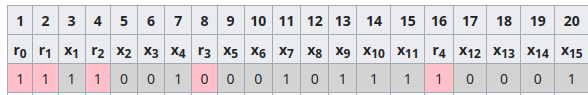
\includegraphics[height=2.1cm]{assets/Hemming_code.png}
\end{center}

\textit{Алгоритм исправления ошибки}: Давайте по полученной строке снова насчитаем контрольные биты по тем же правилам. Теперь давайте найдем индекс изменненого бита. Изначально предположим его равным нулю, начнем проходиться по контрольным битам, если $i$ый насчитанный нами бит не совпадает с тем, что передали нам в строке, то ошибка у нас в числе, у которого в битовой записи на $i$ом месте стоит 1, значит к ответу надо добавить $2^i$. Полученный бит мы просто меняем на противоположный и радуемся. Декодировка также работает за $O(n\log(n))$.

Удивительно, но код Хемминга совпадает с границей Хэмминга, что делает его оптимальным кодированием с исправлением 1 ошибки.

